\subsection{Przykładowa konstrukcja DFA}
Aby przedstawić zachowanie algorytmu, należy rozważyć dane wejściowe bc i bd dla gramatyki
i ATN przedstawione na Rysunku 8.
Symulacja ATN dla decyzji S rozpoczyna subparsery w lewej krawędzi węzłów $p_{S,1}$ i $p_{S,2}$
z początkowymi konfiguracjami $D_0$ $(p_{S,1}, 1, [])$ i $(p_{S,2}, 2, [])$.
Funkcja \textit{closure} dodaje trzy dodatkowe konfiguracje do $D_0$, gdyż „wywołuje” A
z węzłami „powrotu” $p_1$ i $p_3$.
Poniżej przedstawiono DFA wynikające z symulacji ATN względem bc, a następnie bd
(konfiguracje dodane przez \textit{move} zostały zapisane pogrubioną czcionką):
\par
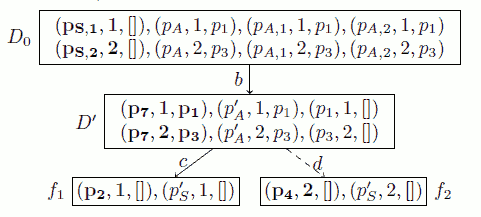
\includegraphics[scale=0.5]{5_4}
\par
Po przewidywaniu bc, DFA posiada stany $D_0$, $D'$, i $f_1$. Ze stanu $D'$ DFA,
\textit{closure} dochodzi do końca A i pobiera ze stosów $\Gamma$, wracając do stanów ATN w S.
Stan $f_1$ jednoznacznie przewiduje numer produkcji na 1. Stan f2 zostaje utworzony i podłączony do DFA
(wskazany przerywaną strzałką) podczas przewidywania drugiej frazy bd.
Funkcja \textit{adaptivePredict} najpierw używa symulacji DFA, aby dojść do $D'$ z $D_0$ względem b.
Przed zobaczeniem bd, $D'$ nie posiada żadnych krawędzi d, tak więc \textit{adaptivePredict}
musi użyć symulacji ATN, aby dodać krawędź $D' \overset{d}{\rightarrow}f_2$

